\chapter[1/f noise in solid-state nanopores is governed by access and surface regions]{1/f noise in solid-state nanopores is governed by access and surface regions}
\chaptermark{1/f noise in nanopores is governed by access and surface regions}
\label{chapter_2}

%% The following annotation is customary for chapter which have already been
%% published as a paper.
\blfootnote{This chapter has been published as: A. Fragasso, S. Pud, and C. Dekker. Nanotechnology 30, 395202 (2019) \cite{Fragasso2019}.}

%% It is only necessary to list the authors if multiple people contributed
%% significantly to the chapter.
%\authors{Albert {\titleshape Einstein}}
%
%%% The '0pt' option ensures that no extra vertical space follows this epigraph,
%%% since there is another epigraph after it.
%\epigraph[0pt]{
%    Nature and nature's laws lay hid in the night; \\
%    God said `Let Newton be!' and all was light.
%}{Alexander Pope}
%
%\epigraph{
%    It did not last: the devil shouting `Ho. \\
%    Let Einstein be!' restore the status quo.
%}{Sir John Collings Squire}

\begin{abstract}
The performance of solid-state nanopores as promising biosensors is severely hampered by low-frequency 1/f noise in the through-pore ionic current recordings. Here, we develop a model for the 1/f noise in such nanopores, that, unlike previous reports, accounts for contributions from both the pore-cylinder, pore-surface, and access regions. To test our model, we present measurements of the open-pore current through solid-state nanopores of different diameters (1-50 nm). To describe the observed trends, it appears essential to include the access resistance in the modelling of the 1/f noise. We attribute a different Hooge constant for the charge carrier fluctuations occurring in the bulk electrolyte and at the pore surface. The model reported here can be used to accurately analyze different contributions to the nanopore low-frequency noise, rendering it a powerful tool for characterizing and comparing different membrane materials in terms of their 1/f-noise properties. 
\end{abstract}

%% Start the actual chapter on a new page.
\newpage


\section{Introduction}
Solid-state nanopores are versatile single-molecule biosensors \cite{Dekker2007}, \cite{Ying2013}, \cite{Shi2018}, \cite{Lin2018} which hold great promise for bio-medical sensing \cite{Atas2012,Squires2013,Miles2012,Sze2017,Yang2018} and sequencing \cite{Merchant2010}. The success of nanopo\-res \cite{Howorka2009,Kasianowicz2008,Deamer2016,Kasianowicz2016} is due to their simplicity and elegant working principle, where upon passing the nanopore, single molecules induce the modulation of the through-pore ionic current, which can be detected by the electronics. Solid-state nanopores, i.e., small pores within a SiN membrane, can efficiently detect the analyte molecules \cite{Wei2012,Kowalczyk2011a}, read-out certain structural features of the detected molecules \cite{Sze2017,Bell2016,Plesa2016}, and even discriminate  short nucleotide sequences \cite{Venta2013}. However, they still lack the precision of their biological counterparts, with which DNA sequencing has been achieved, either by direct reading of DNA bases \cite{Kasianowicz2002,Manrao2012}, or by sequencing-by-synthesis techniques \cite{Kumar2012,Robertson2007,Fuller2016}. This is due to the large translocation speeds \cite{Plesa2013,Storm2005} and the sizeable ionic current noise \cite{Smeets2009}. Indeed, for many applications \cite{Plesa2013,Ketterer2018,Heerema2015} the ionic current noise is a limiting factor.


The ionic current noise in solid-state nanopores originates from multiple sources, \emph{viz.}, the nanopore chip substrate, the membrane dielectric properties, the interface between the nanopore surface and the electrolyte solution, and the bulk of the electrolyte \cite{Uram2008,Smeets2008}. An in-depth overview of noise spectroscopy and its application for nanopore sensors can be found in \cite{Roelen2018,DeFelice1981}. Briefly, the high-frequency part of the ionic current noise arises from capacitance and dielectric loss of the chip \cite{Tabard-Cossa2007} and thus can be engineered to lower values by chip design \cite{Tabard-Cossa2007,Balan2015,Park2016}. On the contrary, there is no established solution to dampen the low-frequency noise, which is mainly characterized by 1/f noise \cite{Smeets2008}, the nature of which is poorly understood. Chen \emph{et al.} \cite{Chen2004} demonstrated that atomically thin films of aluminum oxide deposited onto the nanopore surface  can suppress low-frequency noise in solid-state nanopores, but notably the initial noise that they had as a starting point in their experiments was extremely high as compared to the values commonly measured for bare silicon nitride \cite{Smeets2008,Balan2015}. Smeets \emph{et al.}\cite{Smeets2008} established that 1/f noise in nanopores obeys Hooge's empirical equation which relates the noise to the number of charge carriers in the pore volume. Wen et al. \cite{Wen2017} further investigated the 1/f noise in solid-state nanopores, by analyzing pore-surface and pore-cylinder 1/f noise contributions as a function of pH and salt concentration. However, despite some success in describing the 1/f noise behaviour at different electrolyte conditions, none of these models so far has been able to quantitatively account for the 1/f noise for different nanopore geometries and membrane materials. This lack of a general theory to describe the noise hinders the analysis and search for low-noise nanopore materials and the development of methods for 1/f noise suppression. Indeed, a comprehensive model capable of predicting 1/f noise behavior of solid-state nanopore sensors is very much welcome for further improvement of the sensor ionic-current measurement resolution.


Here, we present a general theoretical noise model for nanopores that, unlike previous reports, accounts for contributions from both the pore-cylinder, pore-surface, and access regions, as indicated in Fig.\ref{fig:sketch}A. Furthermore, we present experimentally measured values of the 1/f noise in SiN solid-state nanopores of different diameters (1-50 nm), and we find an excellent agreement between the model and the data. We show that the dependence of 1/f noise on geometrical parameters of the pores is governed by the distribution of the electric potential between the nanopore and the access region, which has been previously defined \cite{Hall1975} and measured for different nanopore systems \cite{Bezrukov1996,Kowalczyk2011b}. Fitting the model to our experimental data, we deduce that the 1/f noise generated by the bulk (access and pore-cylinder) and surface regions stem from different noise mechanisms and should be described by distinct Hooge constants that differ by more than 3 orders of magnitude. We find that the surface noise dominates the nanopore noise for small pores up to 20 nm in diameter, which emphasizes the importance of surface properties for the nanopore performance. For larger pores, the access resistance dominates the noise properties. Our findings provide a framework for a fair comparison of the low-frequency properties of different membrane materials for nanopore experiments and thus may be of use in the search for new approaches to minimize 1/f noise in solid-state nanopores. 


\begin{figure}
		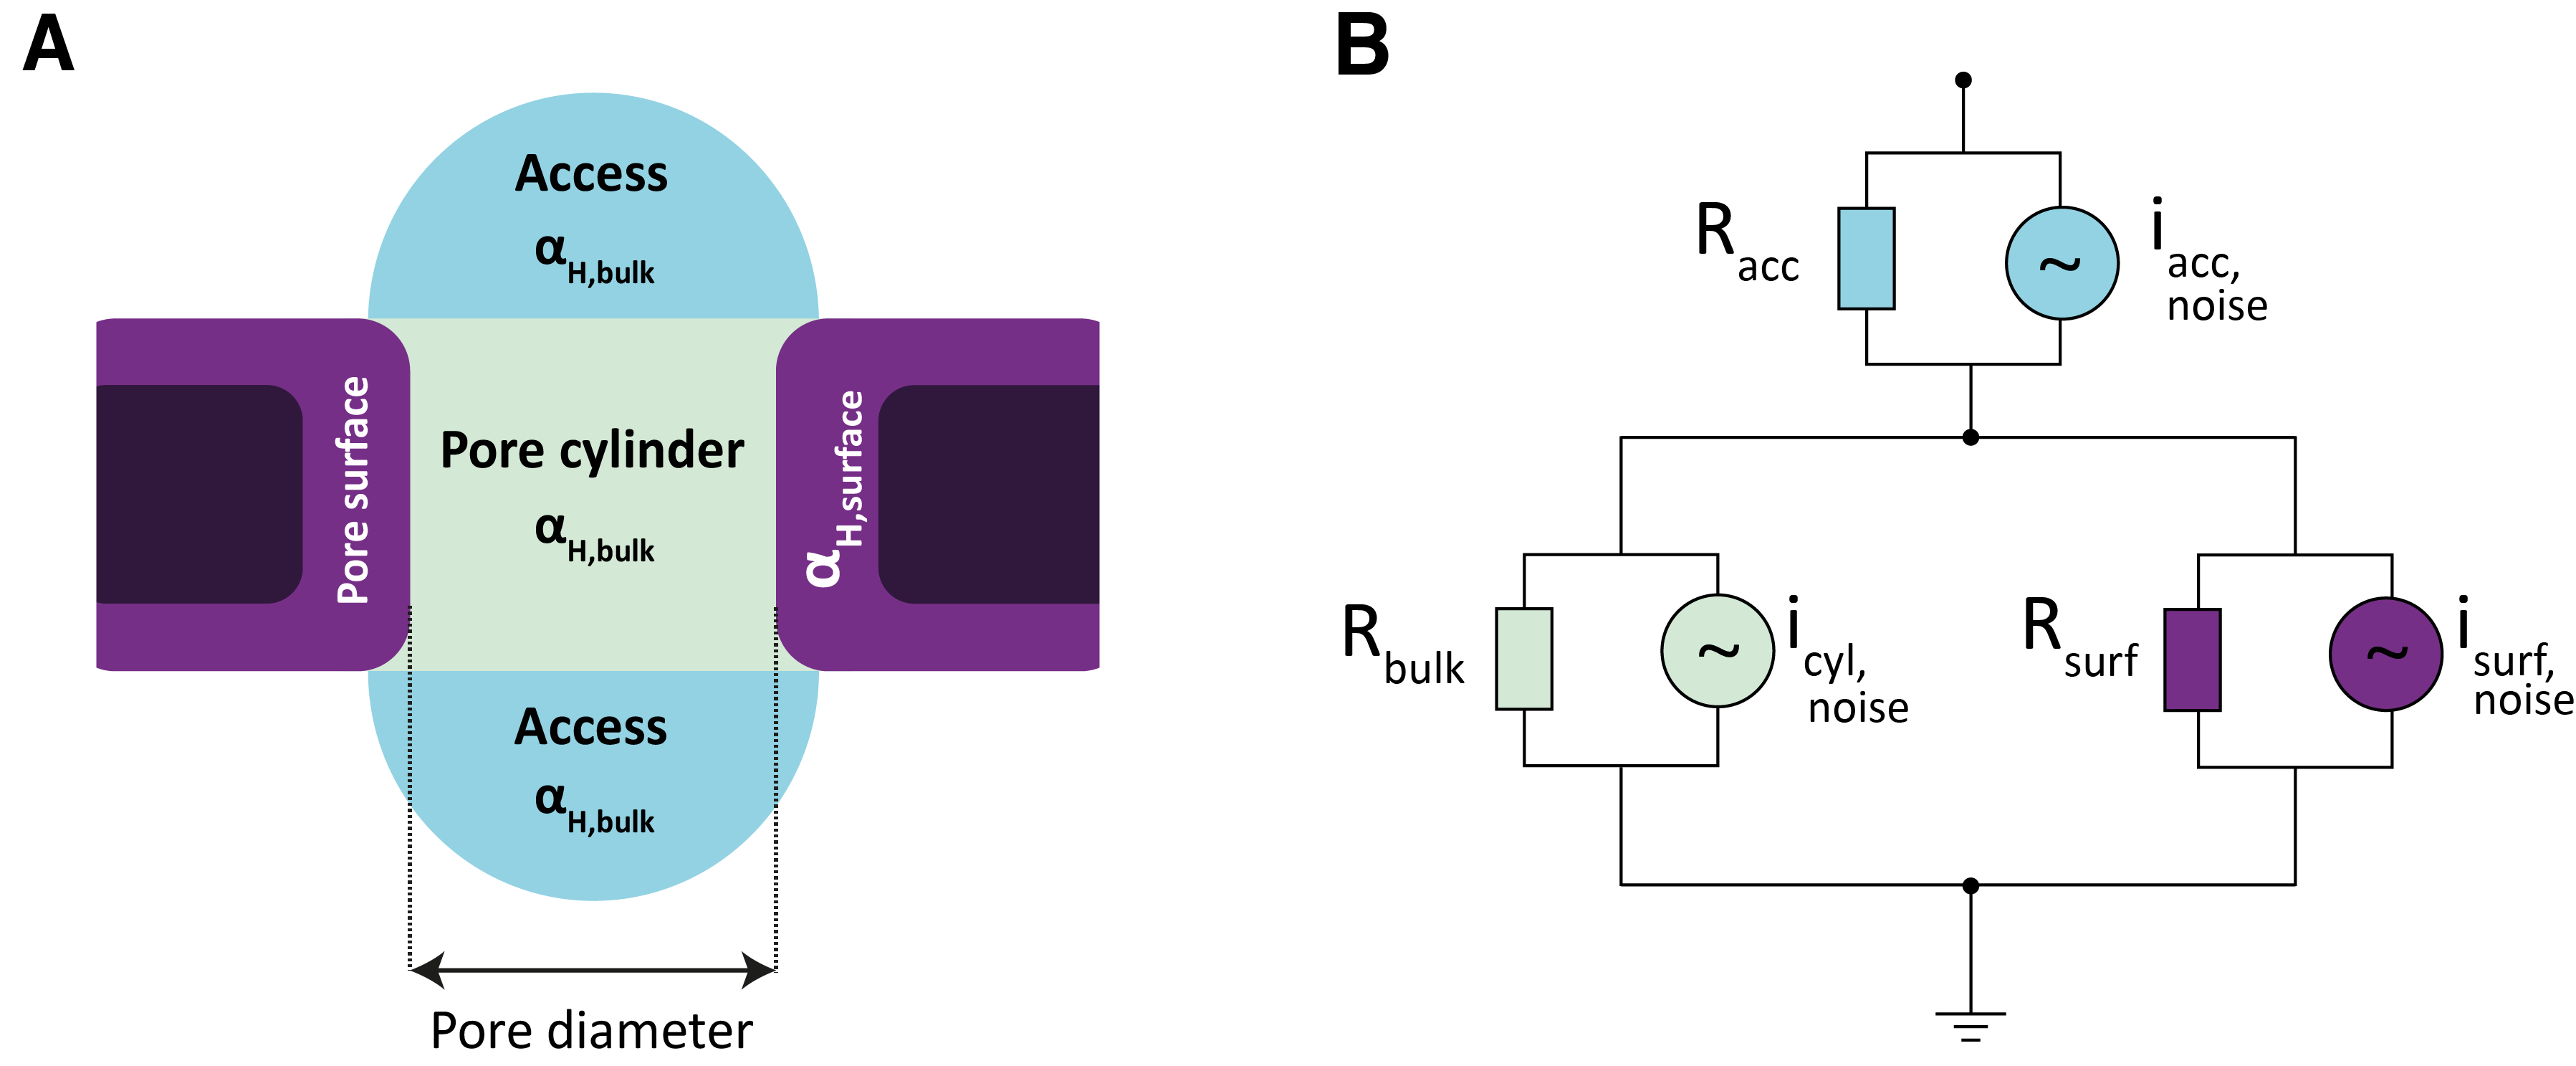
\includegraphics[width=\linewidth]{figures/Figure2.1.png}
		\caption{(A) Schematic representation of the relevant nanopore regions: access region (blue), pore-cylinder region (green), pore-surface (purple). (B) Equivalent circuit of the nanopore sensor. Nanopore regions are modelled as resistive elements connected in parallel to noise current generators.}
		\label{fig:sketch}
\end{figure}

\section{Results}
We develop our model for the low-frequency ionic current noise of the nanopore system based on the equivalent electric circuit of the nanopore, see Fig.\ref{fig:sketch}B. The access region is modelled as a resistor ($R_{acc}$) that is connected in series to the resistances of the pore-cylinder ($R_{cyl}$) and pore surface ($R_{surf}$) that are connected in parallel. $R_{cyl}$ accounts for the dissipative transport of ions in the cylindrical volume of the nanopore, whereas $R_{surf}$ accounts for the contribution of the counterions that are shielding the nanopore surface charge \cite{Smeets2006}. 


We thus define
  
	\begin{align}
	\label{eqn:Eq2.1}
	& R_{pore}= R_{surf} ||R_{cyl}, \\
	\label{eqn:Eq2.2}                       
	& R_{tot}= R_{pore} + R_{acc}.   
  \end{align}

\noindent From basic considerations of ion mobilities and geometry \cite{Kowalczyk2011b}, \cite{Smeets2006}, these resistances  can be expressed as

     \begin{align}
     \label{eqn:Eq2.3}
     & R_{acc}= \frac{1}{ecN_a(\mu_{Cl^-}+\mu_{K^+})d},\\
     \label{eqn:Eq2.4}
     & R_{cyl}=\frac{4L}{\pi ecN_a(\mu_{Cl^-}+\mu_{K^+})d^2}, \\
     \label{eqn:Eq2.5}
     & R_{surf}= \frac{L}{\pi\sigma_{surf}\mu_{K^+}d},
     \end{align}


\noindent where L is the membrane thickness (approximated as $L = 8.6 $nm due to the hourglass shape of the nanopore \cite{Kim2006}), $d$ is the diameter, $e$ is the electron charge, $c$ is the molar concentration of the electrolyte, $N_A$ is the Avogadro’s number, $\mu_{Cl^-}$ and $\mu_{K^+}$ are the carrier mobilities, and $\sigma_{surf}$ is the surface charge density.
Noise sources are modelled as noise-current generators that are connected in parallel to the noiseless resistors. The total current noise power spectra	l density $S_{I,tot}
$ can now be expressed as


\begin{equation}\label{eqn:Eq2.6}
S_{I,tot}=S_{I,acc}\left(\frac{R_{acc}}{R_{tot}}\right)^2+ (S_{I,cyl}+S_{I,surf})\left(\frac{R_{pore}}{R_{tot}}\right)^2 .
\end{equation}

\noindent Derivation of Eq.\ref{eqn:Eq2.6} is a result of application of Kirchoff’s law for the circuit in Fig.\ref{fig:sketch}. In our model for the low-frequency noise, we consider only the 1/f noise for each of the nanopore regions (nanopore cylinder, nanopore surface, access region), which in each case is given by Hooge’s model \cite{Hooge1976}, 


\begin{equation}\label{eqn:Eq2.7}
S_I=\frac{\alpha_H I^2}{N_c f}  
\end{equation}

\noindent where $\alpha_H$ is the Hooge parameter which is an empirical constant that indicates the strength of the 1/f noise, $I$ is the dc current, $N_c$ is the number of charge carriers participating in generating the ionic current, and $f$ is the frequency. By measuring current fluctuations in bulk samples of different metals and semiconductors \cite{Hooge1976}, Hooge found that low-frequency noise stems from fluctuations of sample conductance, which is inversely proportional to the amount of charge carriers. Importantly, this relation was found to suitably describe 1/f noise of the ionic current in solid-state nanopores \cite{Smeets2008}, \cite{Wen2017}. To account for the different contributions to the 1/f noise, the ionic currents and number of charge carriers need to be expressed separately for the three regions.  We define the number of charge carriers present in the access region, $N_{c,acc}$, pore-cylinder region, $N_{c,cyl}$, and pore-surface region, $N_{c,surf}$, as


 \begin{align}
\label{eqn:Eq2.8}
&N_{c,acc}=\pi cN_A\frac{d^3}{6},\\
\label{eqn:Eq2.9}
&N_{c,cyl}=\pi cN_AL\frac{d^2}{4},\\ 
\label{eqn:Eq2.10}
&N_{c,surf}=\pi \sigma_{surf}L\frac{d}{e},   
\end{align}

\noindent where $N_{c,acc}$ is defined as the number of carriers in both hemispherical access regions (as shown in Fig.\ref{fig:sketch}A), which account for most of ($\sim$~95\%) the total 1/f noise occurring in the access regions (details in section \ref{sec:S2.4.6}). Referring to the equivalent circuit model of Figure \ref{fig:sketch}B, we can express the currents for the access $I_{acc}$,  pore-cylinder $I_{cyl}$, and pore-surface $I_{surf}$, simply using Ohm’s law and the voltage divider rule,


 \begin{align}
\label{eqn:Eq2.11}
&I_{acc}=\frac{V}{R_{tot}},\\
\label{eqn:Eq2.12}
&I_{cyl}=\frac{V_{cyl}}{R_{cyl}}= \frac{V}{R_{bulk}}\frac{R_{pore}}{R_{tot}},\\ 
\label{eqn:Eq2.13}
&I_{surf}=\frac{V_{surf}}{R_{surf}}=\frac{V}{R_{surf}}\frac{R_{pore}}{R_{tot}},   
\end{align}


\noindent where V is the applied bias across the entire circuit. $I_{surf}$ represents the current generated by the counterions adjacent to the pore walls. Since the conductance through such layer is different from the pore-cylinder it needs to be accounted as a separate term. To express the total 1/f current noise of the nanopore system, we substitute Equations \ref{eqn:Eq2.11}–\ref{eqn:Eq2.13} into Equation \ref{eqn:Eq2.7} to obtain



 \begin{align}
\label{eqn:Eq2.14}
&S_{I,acc}=\frac{\alpha_H I_{acc}^2}{N_{c,acc}f}=
\frac{\alpha_{H,b}}{N_{c,acc}f}\frac{V^2}{R_{tot}^2},\\
\label{eqn:Eq2.15}
&S_{I,cyl}=\frac{\alpha_H I_{cyl}^2}{N_{c,cyl}f}=
\frac{\alpha_{H,b}}{N_{c,cyl}f}\frac{V^2}{R_{cyl}^2}
\frac{R_{pore}^2}{R_{tot}^2},\\ 
\label{eqn:Eq2.16}
&S_{I,surf}=\frac{\alpha_H I_{surf}^2}{N_{c,surf}f}=
\frac{\alpha_{H,s}}{N_{c,surf}f}\frac{V^2}{R_{surf}^2}
\frac{R_{pore}^2}{R_{tot}^2}.
\end{align}

\noindent Finally, combining Equations \ref{eqn:Eq2.14}–\ref{eqn:Eq2.16} into \ref{eqn:Eq2.6}, we can express the total 1/f noise $S_{I,tot}$ as

\begin{equation}\label{eqn:Eq2.17}
	S_{I,tot}=
	\frac{V^2}{fR_{tot}^4}\frac{\alpha_{H,b} R_{acc}^2}{N_{c,acc}}+
	\frac{V^2}{fR_{tot}^4}\frac{\alpha_{H,b} R_{pore}^4}{R_{cyl}^2N_{c,cyl}}+
	\frac{V^2}{fR_{tot}^4}\frac{\alpha_{H,s} R_{pore}^4}{R_{surf}^2N_{c,surf}}
\end{equation}


\noindent where $\alpha_{H,b}$ and $\alpha_{H,s}$ are the Hooge parameters for the bulk and surface 1/f noise. Note that this model has only two fit parameters $\alpha_{H,b}$ and $\alpha_{H,s}$ whereas all other quantities are given or can be calculated explicitly. 


We experimentally tested this model by carefully examining the dependence of the 1/f noise on nanopore diameter, since the voltage drop over access and inner nanopore regions varies strongly with nanopore diameter Eq.\ref{eqn:Eq2.3}–\ref{eqn:Eq2.5}. We thus prepared and studied a range of solid-state nanopores with sizes from 1.3 nm to 46 nm that were drilled within 20 nm-thick free-standing Si-supported membranes of silicon nitride using a transmission electron microscope (TEM). The details of the fabrication process and experimental setup are described elsewhere \cite{Janssen2012},\cite{VanDenHout2010}. Briefly, the membrane with a drilled nanopore was mounted into a microfluidic flow-cell, such that the nanopore was surrounded by two compartments filled with electrolyte solution. A buffer with 1 M KCl, 10 mM Tris-HCl, 1 mM EDTA, at pH 7 was used for measuring the ionic current through the nanopores. The ionic current through the nanopore was run using Ag/AgCl electrodes connected to an amplifier (Axopatch 200B, Axon Instruments) operating in resistive feedback mode. Current signals were acquired at a bandwidth of 100 kHz and digitized at 250 kHz. All experiments were performed at the room temperature. To ensure consistency, all chips were fabricated from the same wafer and handled equally. Nanopore diameters were calculated from the measured resistance (using Eq.\ref{eqn:Eq2.23}), and generally found to be close (within 5-10\%) to the values measured by TEM imaging (Fig. \ref{fig:fit}A). Nanopores, which were hard to wet or that demonstrated an excessively noisy ionic current baseline (several orders of magnitude larger than across the whole set of nanopores) were excluded from the study. Ionic currents were recorded under a constant 100 mV applied bias. The power spectral density (PSD) of the ionic currents was computed over a time span of up to 60 seconds using a custom-written Matlab script. We fitted the spectra in the low-frequency range (<100 Hz) to extract the 1/f component. All fits were computed using the Matlab Curve Fitting Toolbox.


\begin{figure}
	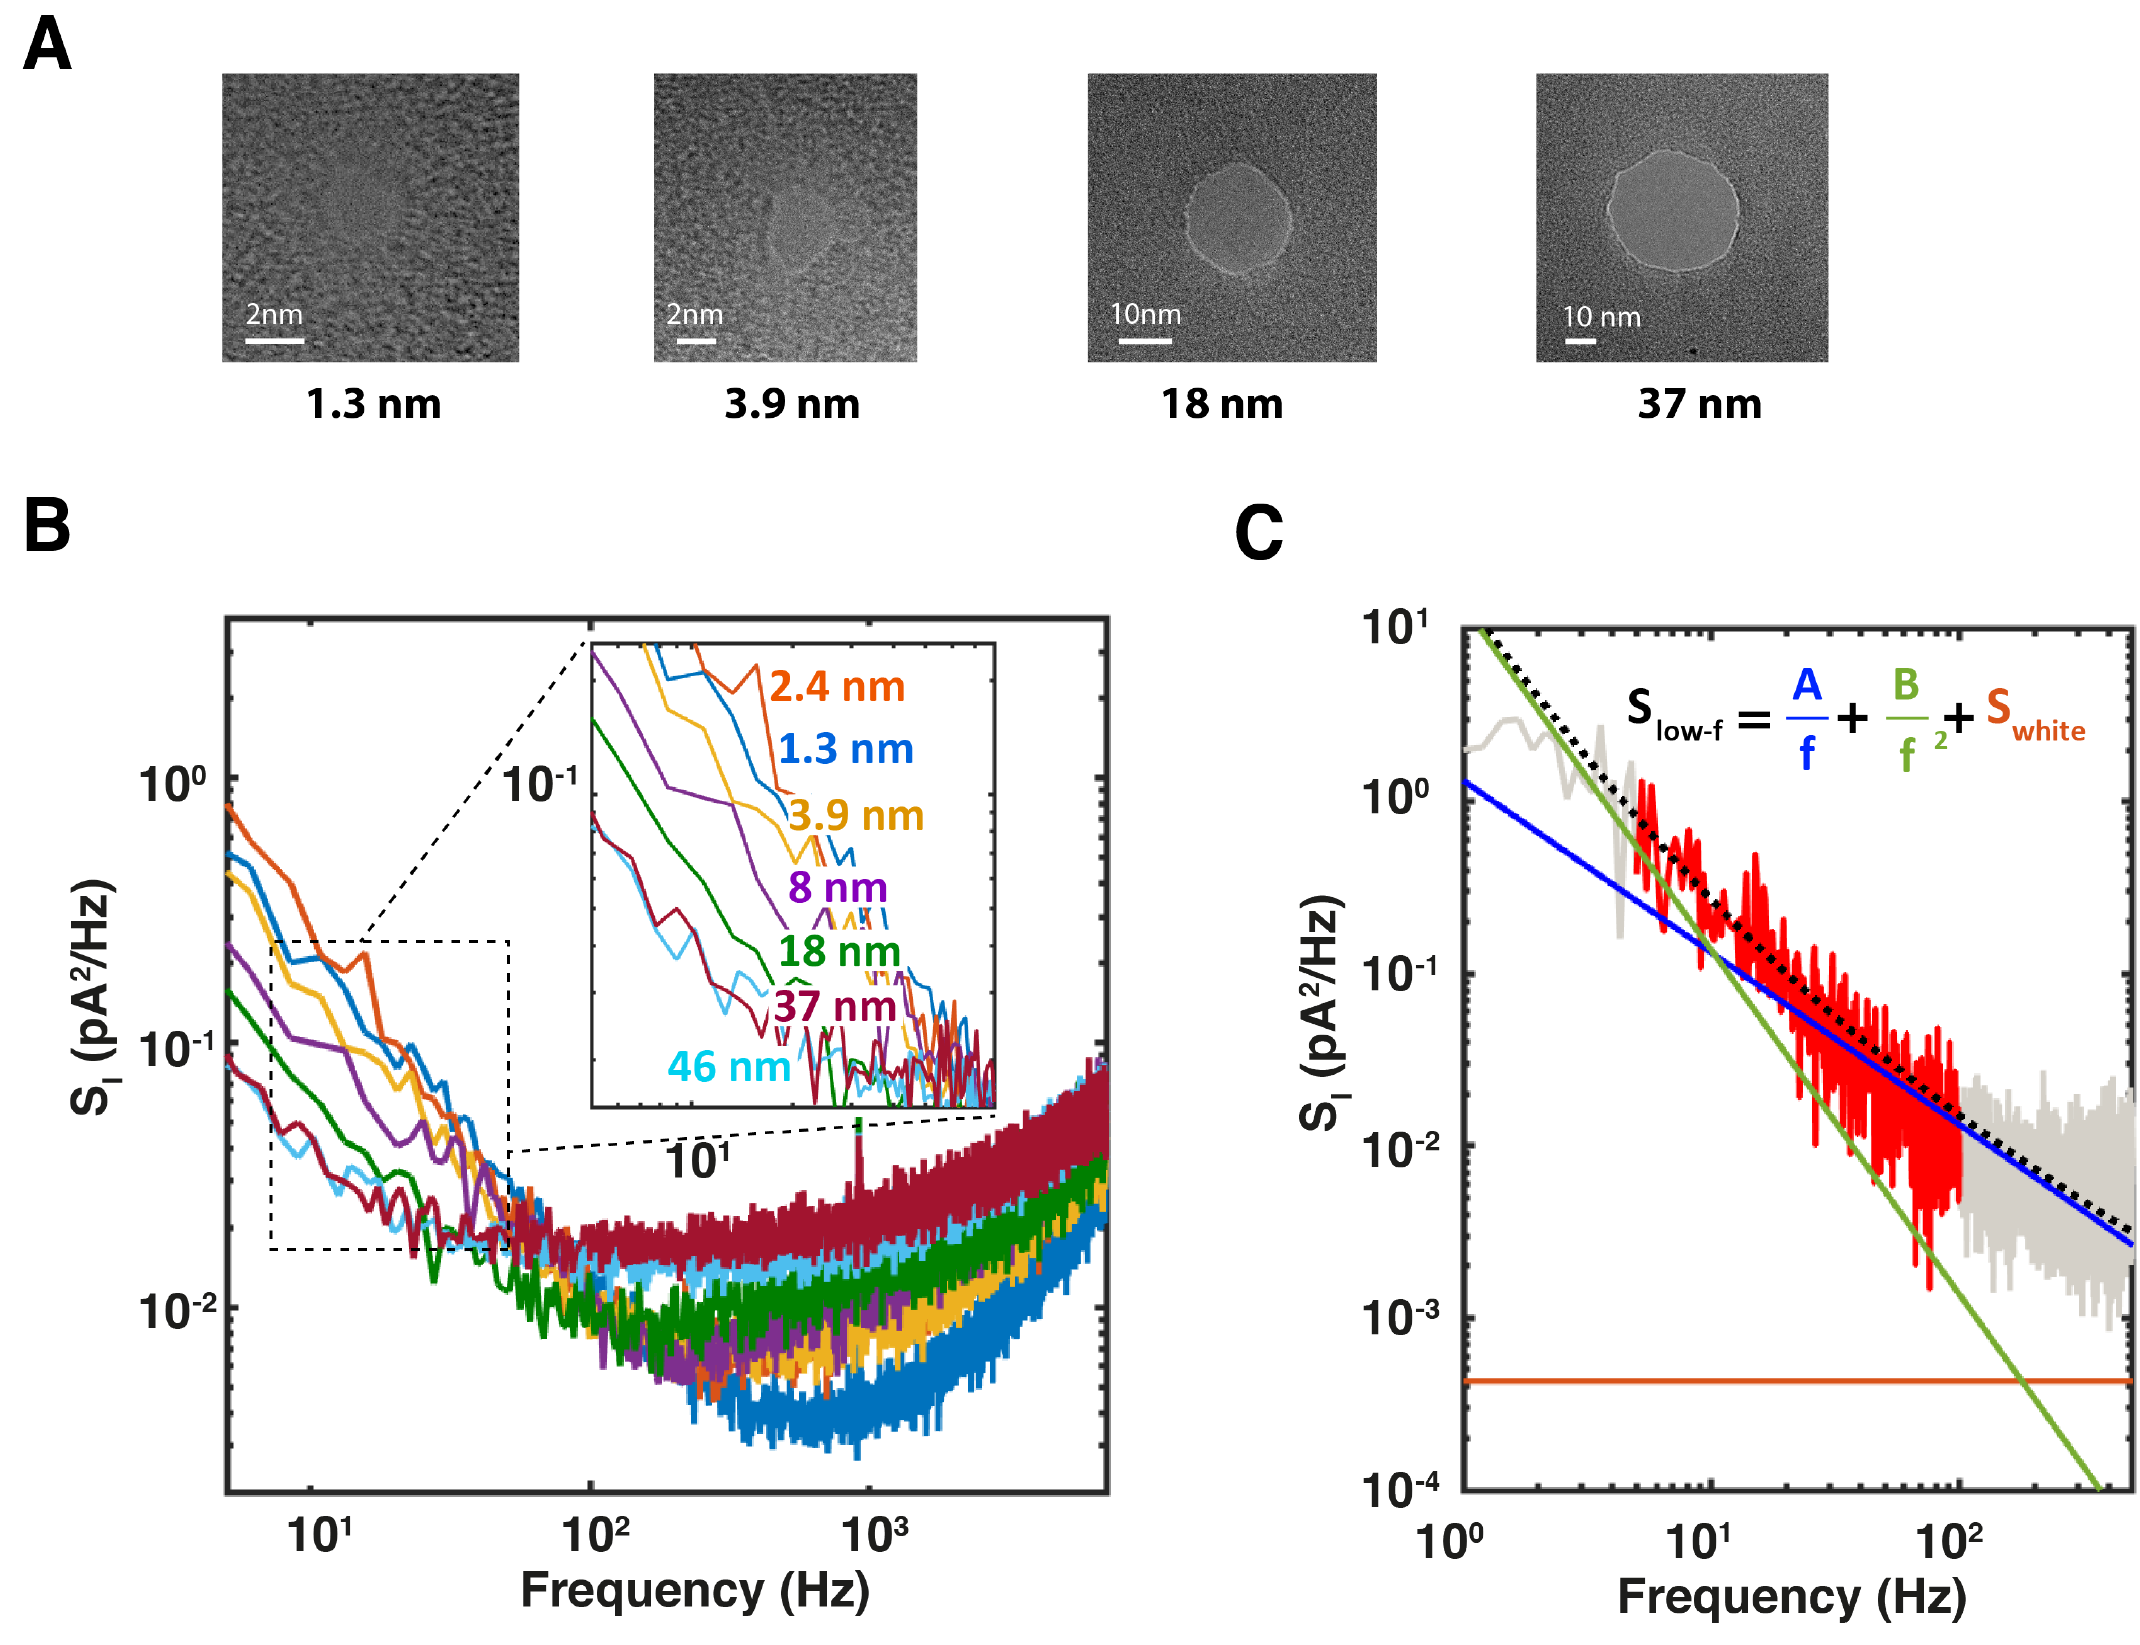
\includegraphics[width=0.95\linewidth]{figures/Figure2.2.png}
	\caption{(A) TEM micrographs of the measured pores. Diameters were calculated from conductance measurements using Eq.\ref{eqn:Eq2.23}. (B) Current power spectral density of nanopores with different diameters between 1.3 and 46 nm. The inset shows a zoom-in of the low frequency regions. (C) Example fit of the low-frequency ionic current power spectral density for a 2.4 nm pore. Dotted black line is the fit to the data (red) as reported by Equation \ref{eqn:Eq2.19}, which comprises 1/f (blue), Lorentzian (green) and white noise (orange) contributions. The rest of the spectrum, out of the fitted region, is shown in light grey. Extracted values of $A$, $B$, and the calculated $S_{white}$ are reported in Table \ref{tab:table2.1}.}
	\label{fig:fit}
\end{figure}

The acquired current power spectral density spectra are shown in Fig.\ref{fig:fit}B. These are characteristic for nanopore noise behavior: at the low-frequency range, the 1/f noise dominates the PSD, then it transitions into a white noise region represented by shot and thermal noise, and subsequently into dielectric and capacitive noise for high-frequencies \cite{Balan2014}. Notably, for pores larger than $\sim$3 nm, the low-frequency noise decreases with increasing nanopore size. On the contrary, the white noise contribution, which we observe in the frequency range from 0.1-1 kHz, increases for larger pores.  This is expected as the white noise, constituted by thermal and shot current noise scales linearly with the conductance $G$ as


\begin{equation}\label{eqn:Eq2.18}
S_{I,white}=S_{I,thermal}+S_{I,shot}=G(4kT+2Vq),
\end{equation}                                          

\noindent where $G$ is the total conductance, $k$ is the Boltzmann constant, $T$ is the absolute temperature in Kelvin (here 290 K), and $q$ is the effective charge of the current carrying species. To extract the magnitude of 1/f noise from the PSD, we used a fitting function constituted by the sum of different low-frequency noise contributions, (Fig.\ref{fig:fit}C), namely


\begin{equation}\label{eqn:Eq2.19}
S_{I,tot}|_{f=1Hz}=S_{I,white}+\frac{A}{f}+\frac{B}{f^2}.
\end{equation} 


\noindent Here, the first term comprises the white noise contributions (\emph{i.e.}, both the thermal and shot noise), the second term represents the 1/f noise, and the third term accounts for a Lorentzian-shaped noise component, which is particularly pronounced in the smaller size nanopores. It can be attributed to fluctuations of the surface charge due to capture/release of ions from the electrolyte onto the nanopore surface \cite{Zhang2018,Bezrukov1993,Hoogerheide2009}. This Loren\-tzian-shaped component is very slow (the characteristic crossover frequency is sub-1Hz) and unlike 1/f noise, is not inherent in all our nanopore data. It is not of major importance but is included in the fits to enable the most accurate determination of the 1/f noise level. Note that the higher-frequency dielectric or capacitive noise contributions are not included into Equation \ref{eqn:Eq2.19} as their magnitude is negligible in the low-frequency range considered. By contrast, the white noise needs to be taken into account, as it is not negligible for the large pores ($>20$ nm) in the 1-100 Hz range (Figure \ref{fig:fig.2.5}).


A major result of the current paper is presented in Fig.\ref{fig:model}A which plots the extracted 1/f noise magnitudes versus nanopore size. We observe a decrease of 1/f noise of almost two orders of magnitude upon going from sub-5 nm pores to $>40$ nm diameter pores. Notably the variation in the 1/f noise is much weaker below a pore size of $\sim$10 nm. To describe this behavior, we first consider previously developed models \cite{Smeets2009}, \cite{Smeets2008}, \cite{Wen2017} that model the 1/f noise as coming only from the cylindrical nanopore, neglecting an access resistance contribution. Following this assumption, the total 1/f noise can be expressed \cite{Wen2017} as

\begin{equation}\label{eqn:Eq2.20}
S_{I,pore}=
\frac{\alpha_{H} I_{surf}^2}{N_{c,surf}f}+
\frac{\alpha_{H} I_{cyl}^2}{N_{c,cyl}f}
\end{equation}

\noindent where the first term describes the pore-surface 1/f noise, the second term describes the pore-cylinder 1/f noise, $\alpha_H$ is the (single) Hooge parameter, and $I_{cyl}$, $I_{surf}$, $N_{c,cyl}$, and $N_{c,surf}$ are calculated explicitly using Equations \ref{eqn:Eq2.9}–\ref{eqn:Eq2.10} and \ref{eqn:Eq2.12}–\ref{eqn:Eq2.13}. Equation \ref{eqn:Eq2.20} describes a monotonic increase of the magnitude of 1/f noise with pore size (for details, see Supporting Information), as illustrated by the green dashed line (Fig.\ref{fig:model}A). Even qualitatively, this clearly contradicts our experimental observations and shows that it is crucial to take the access region into account to describe the size dependence of the 1/f noise. The pink line denotes such a model that accounts for the access resistance, where we have considered the simplest case of an equal Hooge parameter for the 1/f noise from the nanopore bulk and surface, i.e., we fitted Equation \ref{eqn:Eq2.17} to the data with $\alpha_{H,s}=\alpha_{H,b}=\alpha_H$ as the only fit parameter. This model qualitatively describes the trend of the data, but quantitatively clearly fails to fit well. However, by using two different Hooge constants for the 1/f noise at the surface of the nanopore and in the bulk of the electrolyte as fit parameters, an excellent fit to the experimental data can be obtained, as depicted by the purple line. This indicates that 1/f noise arising from the bulk and surface of the nanopore do differ substantially. 

The decrease of the total 1/f noise for increasing pore diameter can be attributed to two underlying causes: (i) a voltage drop redistribution across access and pore region as determined by their resistances (Fig.\ref{fig:sketch}B), which strongly depend on the pore diameter (Eq.\ref{eqn:Eq2.3}–\ref{eqn:Eq2.5}):  whereas the pore resistance dominates for smaller pore diameters, the access resistance dominates for larger pores (Fig.\ref{fig:fig.2.4}); and (ii), the magnitude of 1/f fluctuations is much larger for the surface contribution than for the bulk noise. As a result of these two points, the surface 1/f noise dominates for small pores while the total 1/f noise decreases for larger pores where the weaker access noise dominates. From the fit, we find the surface and bulk Hooge parameters to be $\alpha_{H,s}=(2.1\pm0.2)\cdot10^{-3}$ and $\alpha_{H,b}=(1.4\pm1.5)\cdot10^{-6}$, respectively. Notably, the value we found for the surface noise coefficient is more than three orders of magnitude higher than the bulk value, showing that surface noise dominates. In passing we find it interesting to note that low-frequency noise studies in solid-state semiconductor devices also feature surface currents with a much higher Hooge parameter compared to the bulk ones \cite{Vandamme1994} that arise from fluctuations of electrophoretic mobility of ions in the electrolyte \cite{Jindal1981}. Our value for $\alpha_{H,s}$ is also higher than the value of $\sim1.1\cdot10^{-4}$ published previously for solid-state nanopores \cite{Smeets2008}. However, this value has been extracted using the `pore-only' model and represents a convolution between $\alpha_{H,s}$ and $\alpha_{H,b}$. If we calculate the $\alpha_H$ using a model as in \cite{Smeets2008} for a $\sim$10 nm nanopore from our data set (similar size to the one used in \cite{Smeets2008}), then we find values that agree well with this reference. 


A mechanism responsible for the high surface 1/f noise can possibly be charge carrier number fluctuations occurring at the pore-electrolyte interface due trapping at the surface. Whereas a single adsorption/dissociation process would lead to a Lorentzian noise spectrum,  inhomogeneities at the pore surface will lead to a variety of trapping strengths which yields a 1/f spectrum \cite{Dutta1981}, \cite{Zhang2018}. Such mechanism will strongly depend on the surface properties of the material (in this case SiN\textsubscript{x}). 1/f noise measurements on solid-state nanopores fabricated from two different wafers (Fig.\ref{fig:fig.2.6}) yielded a factor 3 difference in $\alpha_{H,s}$, consistent with this notion. Obviously, our finding of the dominance of surface noise suggests strategies to lower the noise of nanopores, e.g. by surface engineering and choice of surface materials. 


Fig.\ref{fig:model}B sketches the relative contributions of access, pore-cylinder, and pore-surface regions to the total 1/f noise $S_{I,tot}$. Using Eq.\ref{eqn:Eq2.6} and \ref{eqn:Eq2.14}–\ref{eqn:Eq2.17}, the various colored lines plot the access $S_{I,acc}\left(\frac{R_{acc}}{R_{tot}}\right)^2/S_{I,tot}$ (blue), pore-cylinder $S_{I,cyl}\left(\frac{R_{pore}}{R_{tot}}\right)^2/S_{I,tot}$  (green), and pore-surface $S_{I,surf}\left(\frac{R_{pore}}{R_{tot}}\right)^2/S_{I,tot}$   (purple) contributions as a function of pore diameter. Clearly, the 1/f noise for small pores is dominated by surface noise, while for larger pores ($>20$ nm) the noise mainly comes from the bulk noise associated with the nanopore access region. The latter may appear remarkable given that its $\alpha_{H,b}$ is three orders of magnitude lower than $\alpha_{H,s}$, but is explained  by the fact that the access resistance strongly dominates the pore resistance for pore diameters larger than 20 nm.
More generally, our model allows to quantify and predict 1/f noise behavior for nanopores of different geometries. It is clear that ultra-small pores ($<5$ nm) are mainly showing surface 1/f noise and the large ones ($>40$ nm) mainly demonstrate the bulk noise of the access region. However, our model allows to quantify that the mid-range pores, which are most oftenly used for biosensing applications, still have a surprisingly strong contribution from the surface 1/f noise (Fig.\ref{fig:model}B). Therefore, the noise of these pores can be significantly improved by selection of the nanopore material or coating. Moreover, our model is also suitable for nanopores made in ultrathin membranes (e.g. 2D materials) and it predicts a lower 1/f current noise coming from the nanopore itself because of the major role of the access region even for the smaller nanopore diameters. 



	\begin{figure}
		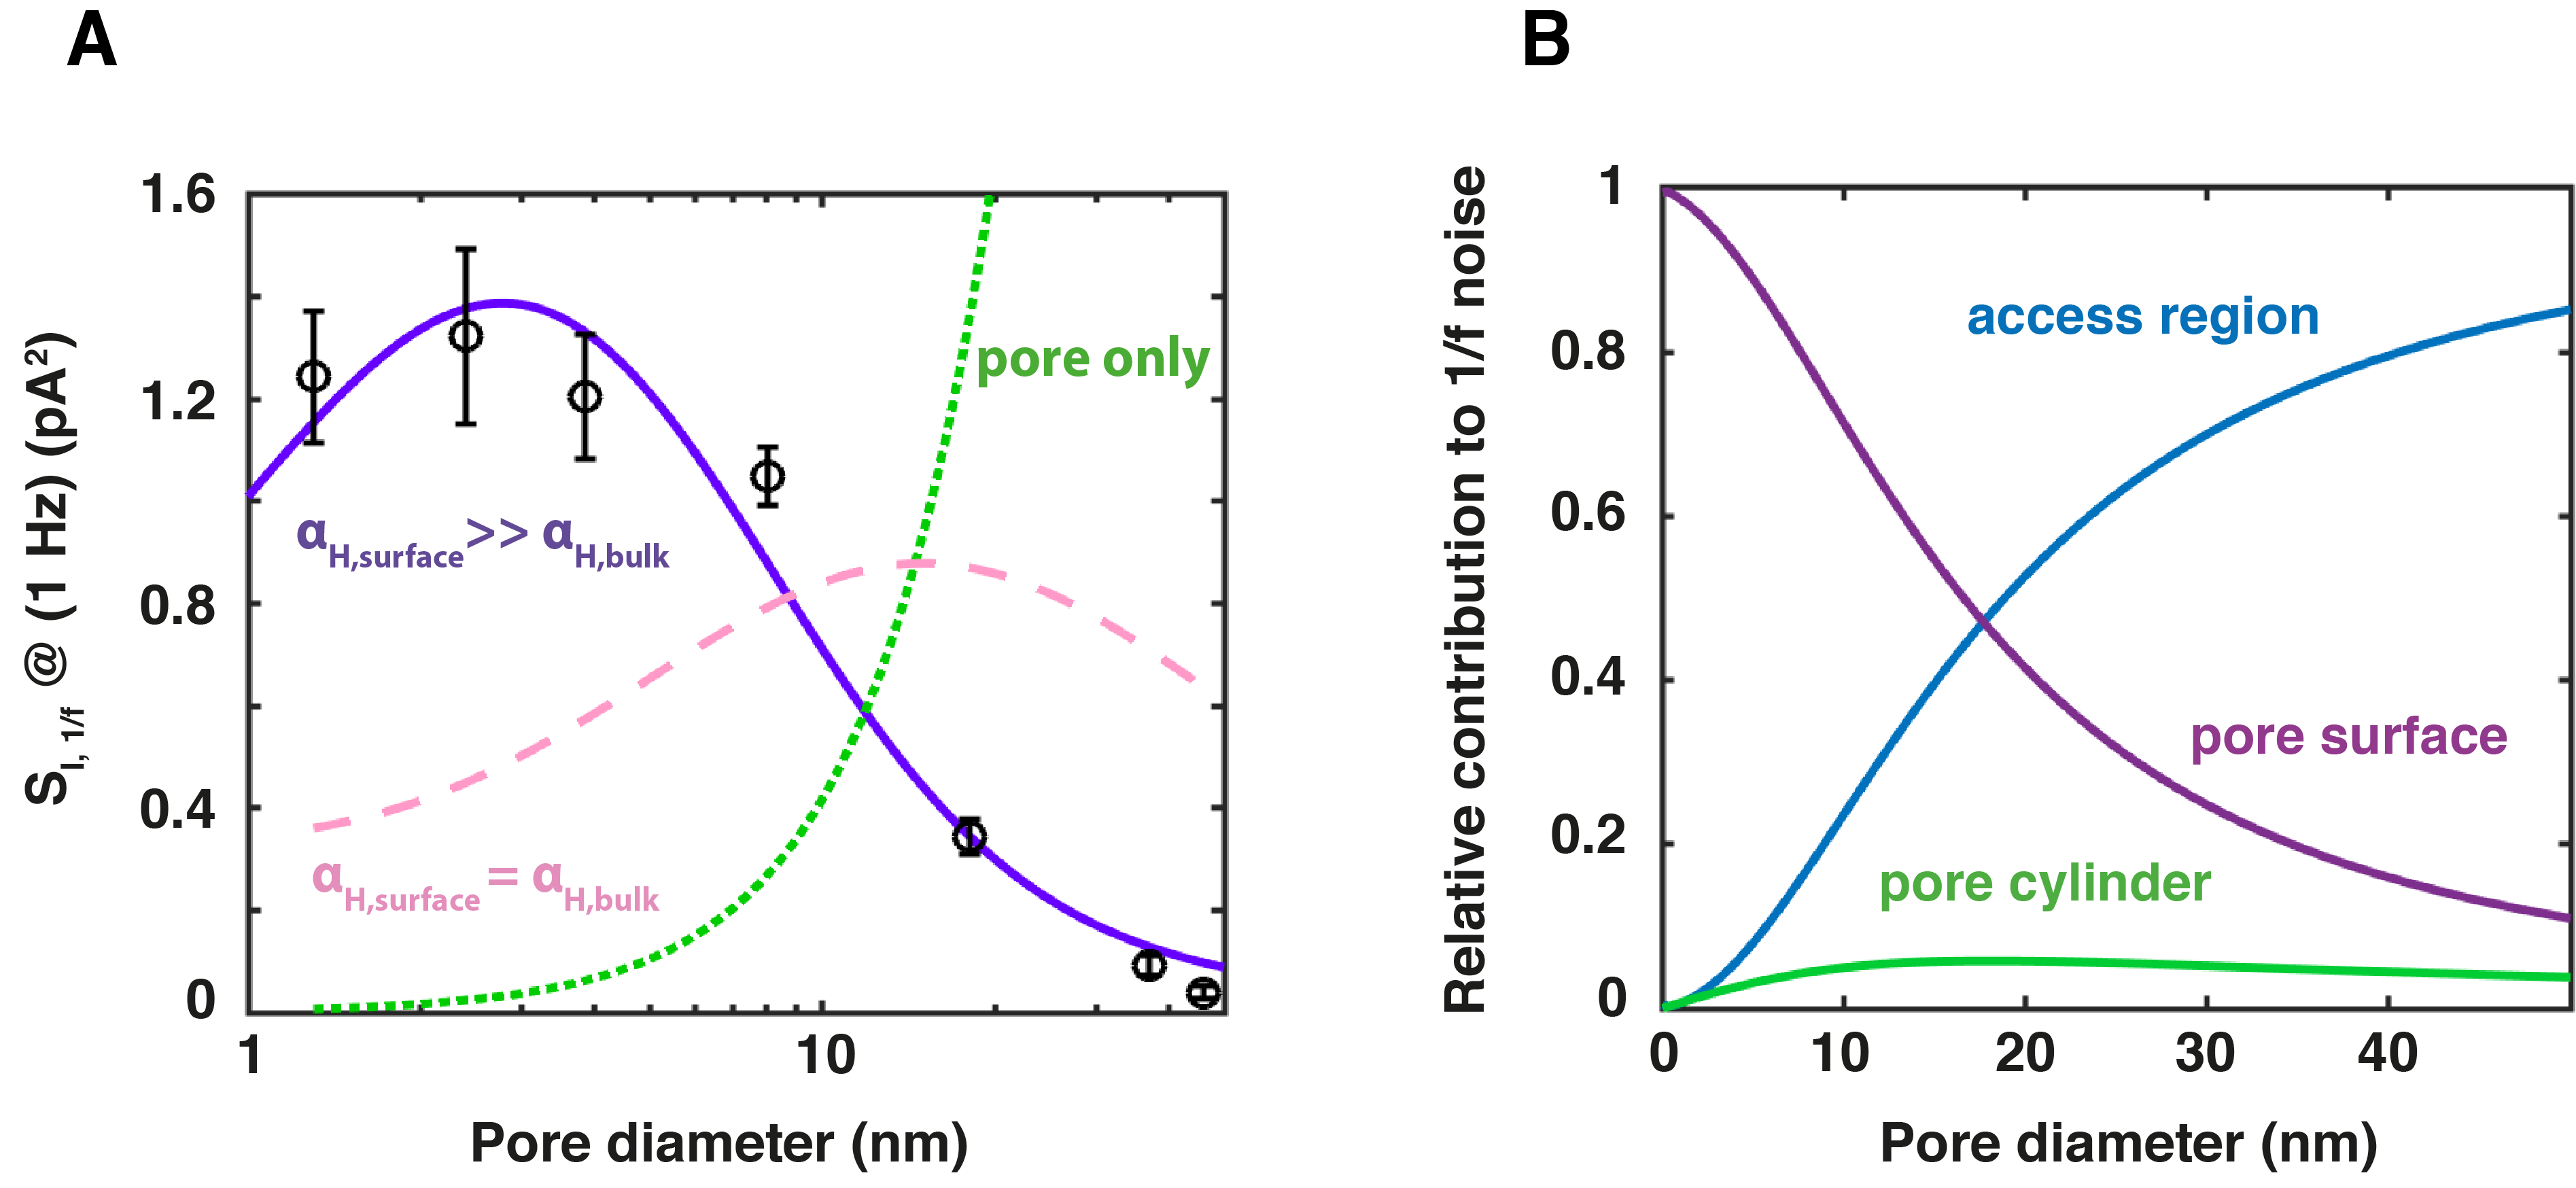
\includegraphics[width=\linewidth]{figures/Figure2.3.png}
		\caption{(A) Low-frequency 1/f noise plotted as a function of the pore diameter (black circles). We observe a decreasing trend of 1/f noise with increasing nanopore size, which spans more than one order of magnitude over the analyzed pore diameter range. Error bars represent standard deviations. The three lines represent model fits to the nanopore data: The green dotted line accounts for the model with no access resistance contribution; pink dashed line includes the access resistance, but treats 1/f noise as coming from one mechanism with a single Hooge parameter; and the purple curve shows the model comprising the access resistance and two independent Hooge parameters associated with bulk and surface noise. (B) Relative contribution to the total 1/f noise originating from the three different nanopore regions: pore-surface (purple), pore-cylinder (green), and access region (blue), as a function of the nanopore diameter.}
		\label{fig:model}
	\end{figure}





\section{Conclusion}


Summing up, we have developed a generalized predictive model for the 1/f noise in solid-state nanopores, which accounts for the dominant role of the access region of the nanopore sensor and for the different origins of 1/f noise in the solid-state nanopore. We find that 1/f noise of a solid-state nanopore derives from two sources, the nanopore surface and the bulk electrolyte, with Hooge parameters that differ by three orders of magnitude. Although the surface noise is more pronounced, the noise coming from the bulk electrolyte in the access region is the predominant source of noise for nanopore diameters larger than 20 nm. The developed model fits the experimental data remarkably well and can thus be used to compare 1/f noise performance of different nanopore materials. Importantly, it may be used to describe the 1/f noise for nanopores in very thin membranes, such as 2D-materials (graphene, boron nitride, molybdenum disulfide), where the access region is reported to dominate also for the smaller pore diameters.


\newpage
\section{Supporting Information}

\renewcommand{\thefigure}{S\thechapter.\arabic{figure}}
\renewcommand{\thetable}{S\thechapter.\arabic{table}}
\renewcommand{\theequation}{S\thechapter.\arabic{equation}}


\subsection{Model}\label{sec:S2.4.1}
From Reference \cite{Kowalczyk2011b,Smeets2006} the $R_{pore}$,$R_{acc}$, and $R_{tot}$ can be expressed as 

\begin{align}
\label{eqn:Eq2.21}
&R_{pore}=R_{cyl} ||R_{surf}=\frac{L}{\pi d} \left[ecN_A(\mu_{Cl^-}+\mu_{K^+})\frac{d}{4}+\sigma_{surf}\mu_{K^+}\right]^{-1},\\
\label{eqn:Eq2.22}
&R_{acc}=\left[ecN_A(\mu_{Cl^-}+\mu_{K^+})d\right]^{-1}\\
\label{eqn:Eq2.23}
&R_{tot}=R_{pore}+R_{acc},
\end{align}

\begin{figure}[h]
	\centering
	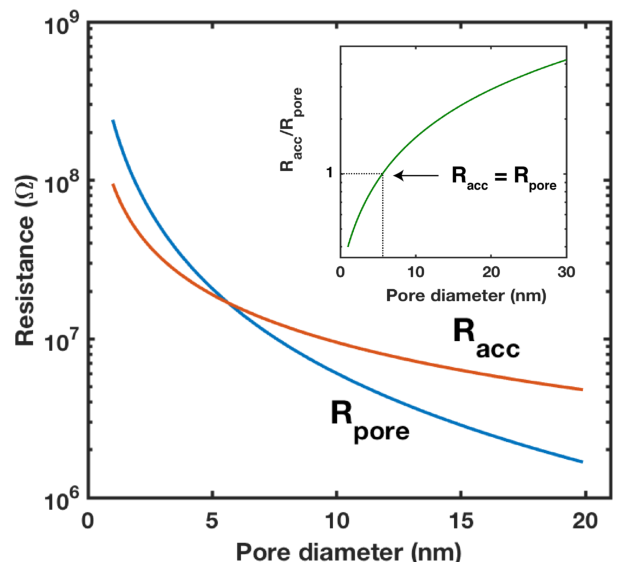
\includegraphics[width=0.6\linewidth]{figures/Figure2.4.pdf}
	\caption{Access and nanopore resistances vs pore diameter. Inset: Ratio of access resistance over nanopore resistance vs pore diameter.}
	\label{fig:fig.2.4}
\end{figure}


\noindent where $L$ is the membrane thickness (assumed to be 8.6 nm, due to the hourglass shape of the nanopore \cite{Kowalczyk2011b}), $d$ is the diameter, $e$ is the charge of the electron, $c$ is the molar concentration, $N_A$ is the Avogadro’s number, $\mu_{Cl^-}$ and $\mu_{K^+}$ the carrier mobilities, and $\sigma_{surf}$ the surface charge density.







\subsection{Fitting the current noise spectral density versus pore diameter}\label{sec:S2.4.2}

To remove one free parameter and improve the goodness of the fit, the analysis was restricted to the frequency region of the spectra where $f\gg f_c$, such that the fit function could be well approximated to



\begin{equation}\label{eqn:Eq2.24}
S_{I,tot}|_{f=1Hz}=\frac{A}{f}+\frac{B'}{1+\left(\frac{f}{f_c}\right)^2}+S_{I,white}\approx\frac{A}{f}+\frac{B}{f^2}+S_{I,white}.
\end{equation} 

\noindent where $B'$ and $f_c$ are factors defining the Lorentzian function, $S_{white}$ was calculated from the pore conductance, and $A$ and $B$ were fit parameters. The results of the fitting of Eq.\ref{eqn:Eq2.24} are illustrated in Figure \ref{fig:fig.2.5}, and the extracted parameters are reported in Table \ref{tab:table2.1}.




\begin{figure}[h]
	\centering
	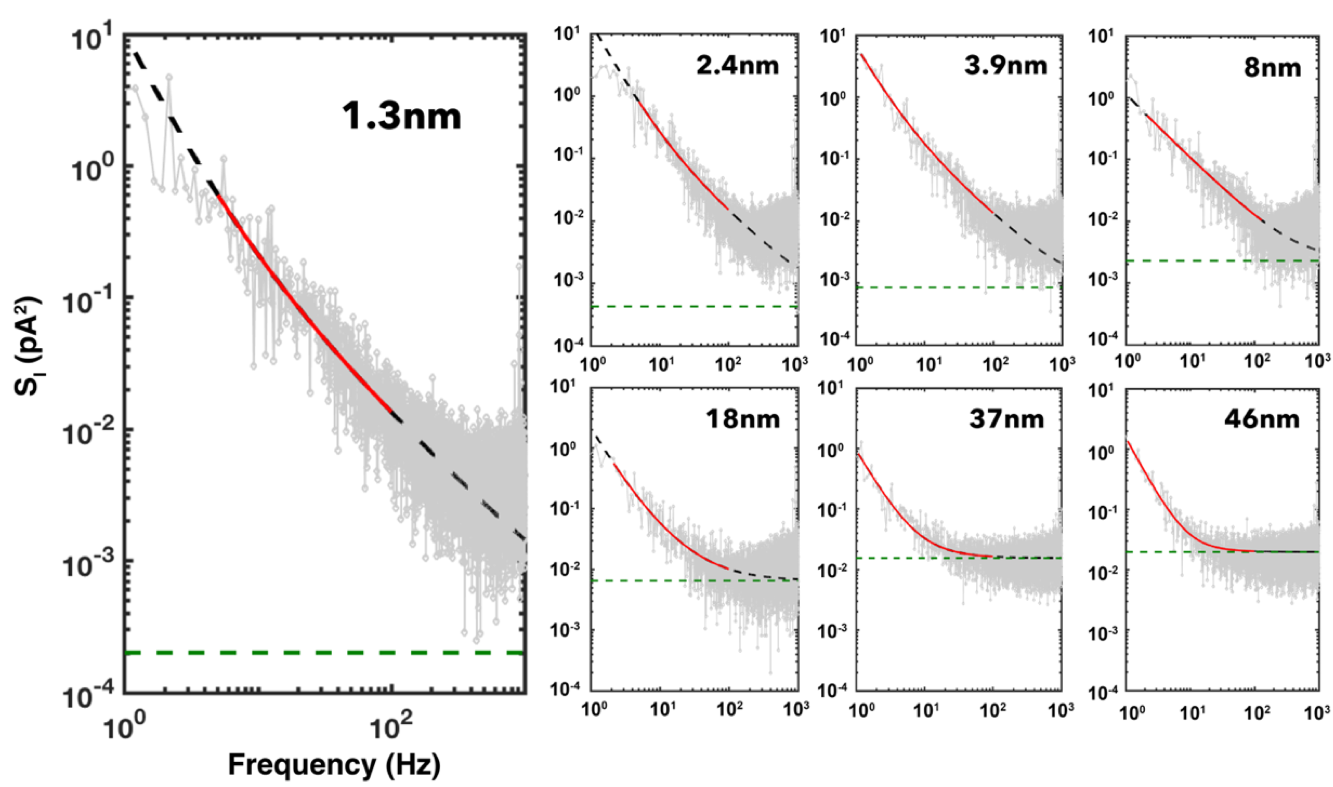
\includegraphics[width=0.95\linewidth]{figures/Figure2.5.png}
	\caption{Current power spectral density for different pore diameters. Black dashed line shows the fit to the data, using Equation \ref{eqn:Eq2.19}. Red line shows the region of the spectrum where the fit was computed. Green dashed line represents the white noise, calculated using Equation \ref{eqn:Eq2.18}.}
	\label{fig:fig.2.5}
\end{figure}



\begin{table}[h]
	\begin{center}
		\begin{tabular}{|c|c|c|c|}
			\hline 
			Pore diameter (nm) & $A$ (pA\textsuperscript{2}) & $B$ (pA\textsuperscript{2} $\cdot$ Hz) & $S_{white}$ (pA\textsuperscript{2}/Hz)\\
			\hline 
			\centering
			1.3 & $1.24\pm 0.13$ & $8.8\pm  1.1$  & $2.9\cdot10^{-4} $ \\
			2.4 & $1.32\pm 0.17$ & $13.7\pm 1.4$  & $4.3\cdot10^{-4} $ \\
			3.9 & $1.21\pm 0.12$ & $5.62\pm 0.23$ & $8.5\cdot10^{-4} $ \\
			8   & $1.05\pm 0.06$ & $0.11\pm 0.19$ & $2.3\cdot10^{-3} $ \\
			18  & $0.34\pm 0.03$ & $1.82\pm 0.10$ & $6.5\cdot10^{-3} $ \\
			37  & $0.09\pm 0.02$ & $0.84\pm 0.03$ & $15.4\cdot10^{-3}$ \\
			46  & $0.04\pm 0.01$ & $1.50\pm 0.02$ & $19.7\cdot10^{-3}$ \\
			\hline 
		\end{tabular}
	  \caption{\label{tab:table2.1}Fit parameters for different pore diameters. $A$ and $B$ were free parameters. $S_{I,white}$ was calculated from the measured conductance and the voltage applied according to Equation \ref{eqn:Eq2.18}.}
	\end{center}
\end{table}




\subsection{Fitting 1/f noise versus diameter with the alternative models}\label{sec:S2.4.3}


\subsubsection{Fitting the ‘pore only’ model}


The green dashed line in Figure \ref{fig:model}A represents a 1/f noise model where the access resistance is omitted. In such a scenario, Equations \ref{eqn:Eq2.9}–\ref{eqn:Eq2.10} and \ref{eqn:Eq2.12}–\ref{eqn:Eq2.13} are still used to express the number of charge carriers and currents for the surface and bulk regions. However, the total 1/f noise $S_{I,pore}$ expression would differ from Equation \ref{eqn:Eq2.17}, as in this case 


\begin{equation}\label{eqn:Eq2.25}
S_{I,pore}=S_{I,cyl}+S_{I,surf}.
\end{equation}


\noindent Substituting Eq.\ref{eqn:Eq2.12}–\ref{eqn:Eq2.13} into Eq.\ref{eqn:Eq2.7} and into \ref{eqn:Eq2.25}, and noting that $R_{tot}=R_{pore}$, one gets

\begin{equation}\label{eqn:Eq2.26}
S_{I,pore}=\frac{\alpha_HI_{cyl}^2}{N_{c,cyl}f}+\frac{\alpha_HI_{surf}^2}{N_{c,surf}f}=\frac{\alpha_HV^2}{f}\left[\frac{1}{N_{c,cyl}R_{cyl}^2}+\frac{1}{N_{c,surf}R_{surf}^2}\right].
\end{equation}





\noindent Note that here only one Hooge constant $\alpha_H$ is taken to describe both the bulk and surface contributions. From Eq. \ref{eqn:Eq2.4}–\ref{eqn:Eq2.5} and \ref{eqn:Eq2.9}–\ref{eqn:Eq2.10} we can extract the scaling for $R_{cyl}$, $R_{surf}$, $N_{c,cyl}$, and $N_{c,surf}$ as a function of the pore diameter $D$.

\begin{align}
\label{eqn:Eq2.27}
&R_{cyl}=\frac{4L}{\pi ecN_A(\mu_{Cl^-}+\mu_{K^+})D^2}\propto d^{-2},\\
\label{eqn:Eq2.28}
&R_{surf}=\frac{L}{\pi \sigma_{surf}\mu_{K^+}D}\propto d^{-1},\\
\label{eqn:Eq2.29}
&N_{c,cyl}=\pi cN_AL\frac{d^2}{4}\propto d^2,\\
\label{eqn:Eq2.30}
&N_{c,surf}=\pi \sigma_{surf}L\frac{d}{e}\propto d.
\end{align}


\noindent We can thus rewrite Eq.\ref{eqn:Eq2.26} as 

\begin{equation}\label{eqn:Eq2.31}
S_{I,pore}=  p\cdot d^2+\cdot d,
\end{equation}

\noindent where $p$ and $q$ are constants. This explains the monotonic increasing behavior observed in Figure \ref{fig:model}A for the green dotted line. 



\subsubsection{ Fitting the ‘$\alpha_{H,s}=\alpha_{H,b}$’ model}


The pink dashed curve in Figure \ref{fig:model}A is obtained by fitting the model described by Equation \ref{eqn:Eq2.17} with only one fit Hooge parameter $\alpha=\alpha_{H,s}=\alpha_{H,b}$, which was found to be $\alpha=(1.2\pm 1.0)\cdot 10^{-5}$. 



\begin{table}[h]
	\begin{tabular}{|l|c|c|}
		\hline
			Parameter & Value & Ref.\\
			\hline
			Effective membrane thickness $L$ & $8.6$ nm &\cite{Kowalczyk2011b}  \\
			Potassium ion mobility $\mu_{K^+}$  & 7.616 $\cdot 10^{-8} \left[\frac{m^2}{ V\cdot s}\right]$ & \cite{Lide2005}  \\
			Chloride ion mobility $\mu_{Cl^-}$  & 7.909 $\cdot 10^{-8} \left[\frac{m^2}{ V\cdot s}\right]$ &\cite{Lide2005}   \\
			Surface charge density for Si\textsubscript{3}N\textsubscript{4} at pH 7-8, $\sigma_{surf} $ &  $0.02 \left[\frac{C}{m^2}\right]$&\cite{Sonnefeld1996}   \\
			Bulk conductivity at 1 M KCl $\sigma_{bulk}$ & 10.5 $\left[\frac{S}{m}\right]$ & \cite{Haynes2010}\\
		\hline
	\end{tabular}
\caption{\label{tab:table2.2}Parameters used.}
\end{table}



\subsection{Wafer-to-wafer variability of $\alpha_{H,s}$}\label{sec:S2.4.4}

\begin{figure}[H]
	\centering
	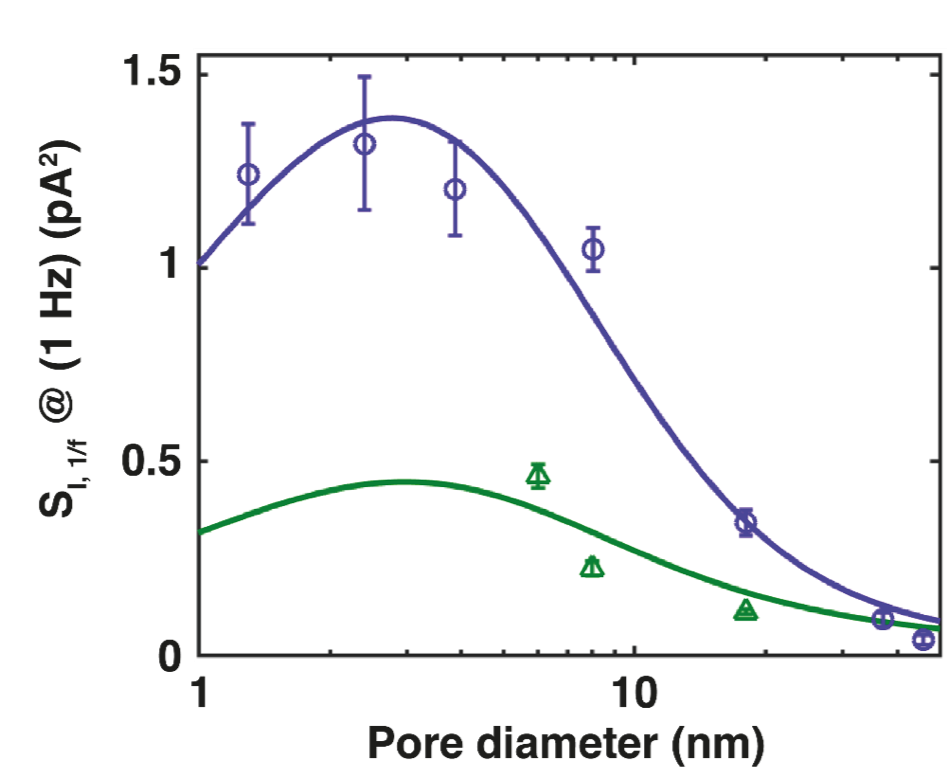
\includegraphics[width=0.7\linewidth]{figures/Figure2.6.png}
	\caption{Low-frequency 1/f noise plotted as a function of the pore size. Nanopores fabricated from different wafers display different surface Hooge constant. We find $\alpha_{H,s}=(2.1\pm 0.2)\cdot 10^{-3}$ for the first batch of pores (purple circles), whereas $\alpha_{H,s}=(6.6\pm 3.4)\cdot 10^{-4} $for the second one (green triangles). Purple and green curves represent the model fitting the 1/f noise data. Error bars represent standard deviations due to the fitting.}
	\label{fig:fig.2.6}
\end{figure}



\subsection{Other noise sources}\label{sec:S2.4.5}

\subsubsection{Background noise}

\begin{figure}[ht]
	\centering
	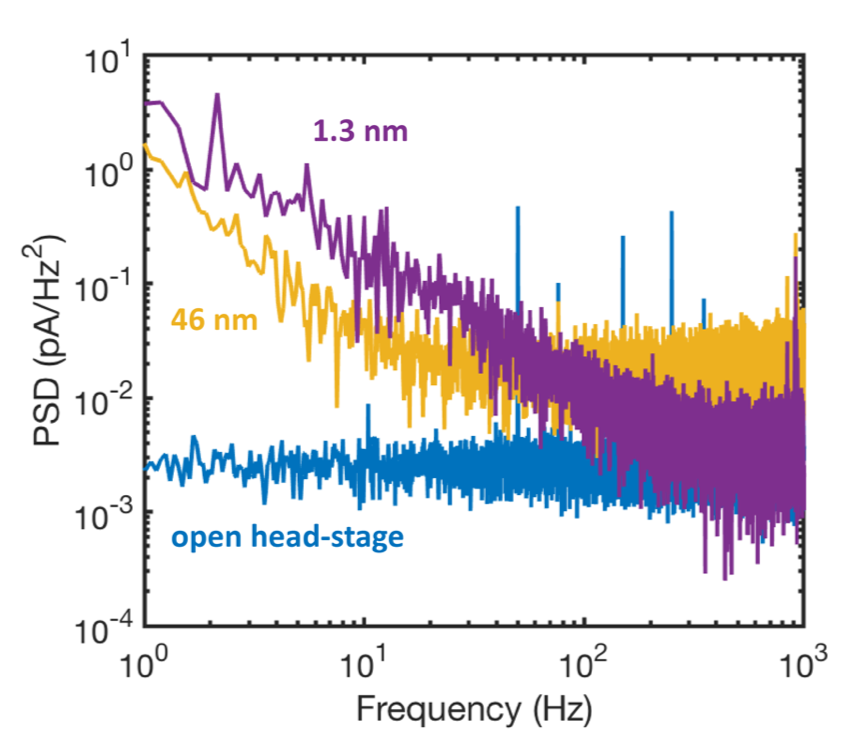
\includegraphics[width=0.7\linewidth]{figures/Figure2.7.png}
	\caption{Comparison of PSD spectra for 1.3 nm (purple) and 46 nm (yellow) vs background noise (blue) coming from the open head-stage of the amplifier. We find the background noise to be at least an order of magnitude lower than the 1/f noise coming from the nanopores in the frequency range of interest (1-100 Hz).}
	\label{fig:fig.2.7}
\end{figure}

\subsubsection{Dielectric noise}
In the frequency range 3-10 kHz, dielectric noise can be  fitted using the linear function
\begin{equation}\label{eqn:Eq2.32}
S_{dielectric}=8\pi kTDC_{chip}f=a\cdot f 
\end{equation}

\noindent where $kT=4.11\cdot10^{-21}J$ at room temperature, $D$ is the dielectric loss, $C_{chip}$ is the chip capacitance, $f$ is the frequency, and $a$ is the fit parameter, found to be $a=(5.03\pm 0.01)\cdot 10^{-6}$ (pA/Hz)\textsuperscript{2}. We find the dielectric noise contribution to be negligible, being more than one order of magnitude lower in the frequency range of interest (1-100 Hz). 


\begin{figure}[H]
	\centering
	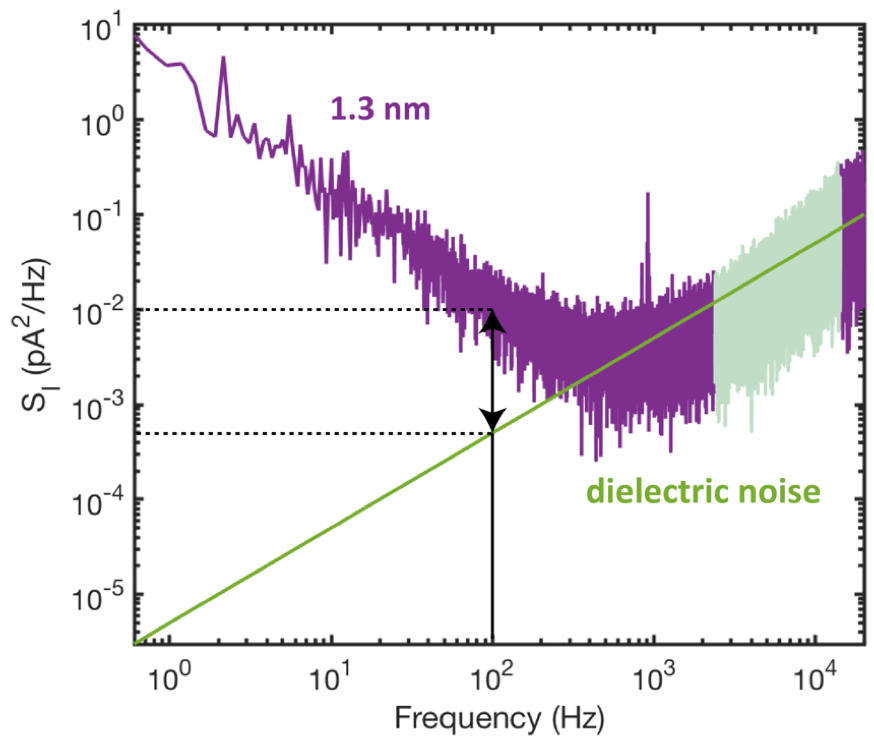
\includegraphics[width=0.7\linewidth]{figures/Figure2.8.png}
	\caption{PSD spectrum of the ionic current for a 1.3 nm pore (purple) with a fit to the dielectric noise (light green,3-10 kHz). Green straight line represents the fit. Dielectric noise was fitted using Equation \ref{eqn:Eq2.32}. Arrows and dashed lines highlight that dielectric noise is negligible in the frequency range of interest (1-100 Hz).}
	\label{fig:fig.2.8}
\end{figure}

\subsection{1/f noise in the access region}\label{sec:S2.4.6}

In this section, we estimate what volume of the access region contributes most to the 1/f noise. Using the formalism developed by Hille \cite{Hille1968}, we derive the amount of 1/f noise coming from the infinite region outside the hemisphere of nanopore radius (Figure \ref{fig:fig.2.9}A). We define the total $S_V$ coming from this region as $S_{V_inf}$. To quantify this value, one can imagine the space as a series connection of hollow hemispheres of electrolyte solution, each with the thickness of $dr$ (Figure \ref{fig:fig.2.9}B). Since all the hollow hemispheres are connected in series, the total voltage PSD is a sum of voltage PSD’s of all hollow hemispheres $dS_{V_{inf}}$. The voltage PSD of hollow hemisphere can be defined as follows:

\begin{equation}\label{eqn:Eq2.33}
dS_{V_{inf}}=dS_{I_{inf}}R_{hh}^2=\frac{\alpha_HI^2}{fN_{hh}}R_{hh}^2,
\end{equation}


\noindent where $R_{hh}$ is the resistance of the hollow hemisphere:

\begin{equation}\label{eqn:Eq2.34}
R_{hh}=\frac{1}{\sigma}\frac{dr}{2\pi r^2},
\end{equation}

\noindent and $N_hh$ is the amount of charge carriers in the hollow hemisphere:

\begin{equation}\label{eqn:Eq2.35}
N_{hh}=cN_A2\pi r^2dr.
\end{equation}
        
\noindent Substituting these values yields the final differential form of $dS_{V_{inf}}$:

\begin{equation}\label{eqn:Eq2.36}
dS_{V_{inf}}=\frac{\alpha_HI^2}{8fcN_A\pi^3 \sigma^2 }\frac{dr}{r^6}.
\end{equation}


\noindent Finally, the total $S_{V_{inf}}$ is derived by integration of $dS_{V_{inf}}$ from the pore radius to infinity

\begin{equation}\label{eqn:Eq2.37}
dS_{V_{inf}}=\frac{\alpha_HI^2}{8fcN_A\pi^3 \sigma^2 }\int_{r_{pore}}^{\infty}\frac{dr}{r^6}=\frac{\alpha_HI^2}{40fcN_A\pi^3 \sigma^2 r_{pore}^5}.
\end{equation}
                                   
\noindent These calculations do not take into account the region within the hemisphere of the pore radius (the volume of electrolyte closest to the pore). To quantify this, we need to derive the resistance and amount of carriers within this hemisphere:

\begin{equation}\label{eqn:Eq2.38}
S_{V_{hemisphere}}=\frac{\alpha_HI^2}{fN_{hemisphere}}R_{hemisphere}^2.
\end{equation} 

\noindent The resistance of the hemisphere of the nanopore radius can be calculated as a difference between resistances of the access region derived using Hall \cite{Hall1975}and Hille \cite{Hille1968} models (Figure \ref{fig:fig.2.9})

\begin{equation}\label{eqn:Eq2.39}
R_{hemisphere}=R_{Hall}-R_{Hille}=\frac{1}{4\sigma r_{pore}}-\frac{1}{4\pi \sigma r_{pore}}=\frac{\pi-1}{4\pi\sigma r_{pore}}.
\end{equation}               

\noindent The amount of carriers within the hemisphere is given by:

\begin{equation}\label{eqn:Eq2.40}
N_{hemisphere}=cN_A\frac{2}{3}\pi r_{pore}^3 .
\end{equation}   


\noindent Therefore the 1/f noise within the hemisphere is:

\begin{equation}\label{eqn:Eq2.41}
S_{V_{hemisphere}}=\frac{3\alpha_HI^2(\pi-1)^2}{32fcN_A\pi^3\sigma^2r_{pore}^5}.
\end{equation} 





\begin{figure}[!htb]
	\centering
	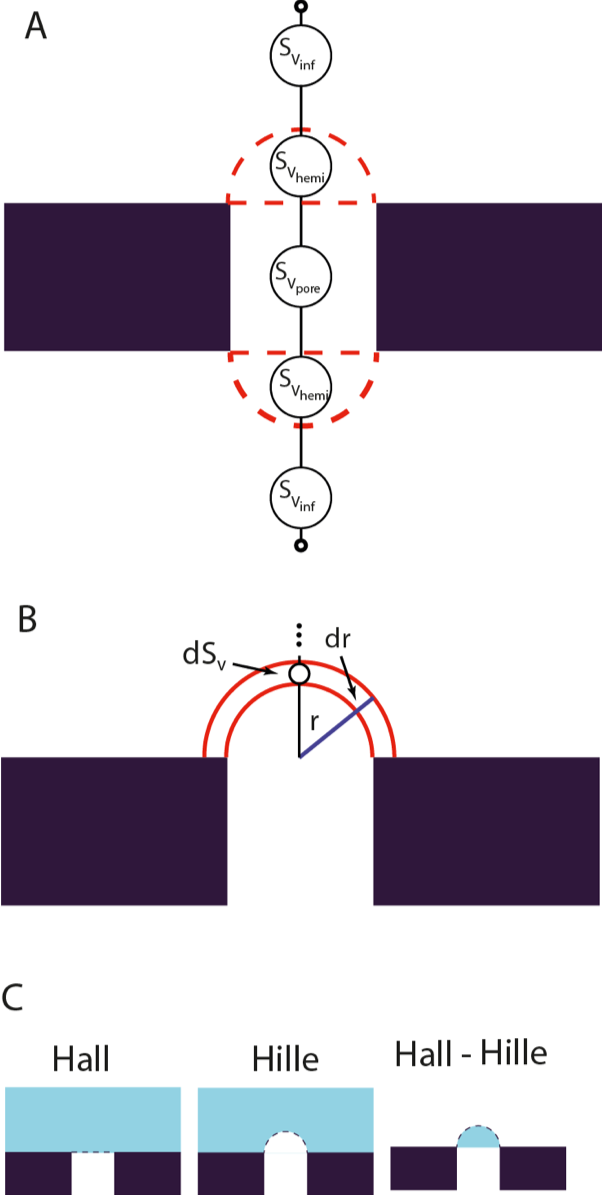
\includegraphics[width=0.5\linewidth]{figures/Figure2.9.png}
	\caption{A. Representation of total voltage PSD of a nanopore sensor as an equivalent circuit with voltage generators defined by nanopore region, hemisphere around the nanopore, infinite space of the electrolyte. B. Schematic to illustrate the representation of voltage PSD of 1/f noise in the infinite bulk solution as a sum of voltage PSD’s of hollow hemispheres. C. Illustration of the volumes considered by Hall and Hille models of the access regions. Blue color indicates the volume taken into account for estimation of the access resistance.}
	\label{fig:fig.2.9}
\end{figure}

\noindent Now we can analytically derive which part of the access region contributes most to 1/f noise:

\begin{equation}\label{eqn:Eq2.42}
\frac{S_{V_{hemisphere}}}{S_{V_{hemisphere}}+S_{V_{inf}}}=\frac{\frac{3(\pi-1)^2}{32}}{\frac{3(\pi-1)^2}{32}+\frac{1}{40}}\approx 0.95.
\end{equation} 



\noindent We conclude that 95\% of the 1/f noise of the access region derives from the hemisphere directly adjacent to the pore. 


\subsection{1/f noise vs voltage applied on a 45 nm pore}\label{sec:S2.4.7}


PSD spectra of the ionic current were acquired at different excitation voltages (20-100 mV) for a 45 nm pore. We find that, as expected, the 1/f noise increases with the square of the current.

\begin{figure}[!htb]
	\centering
	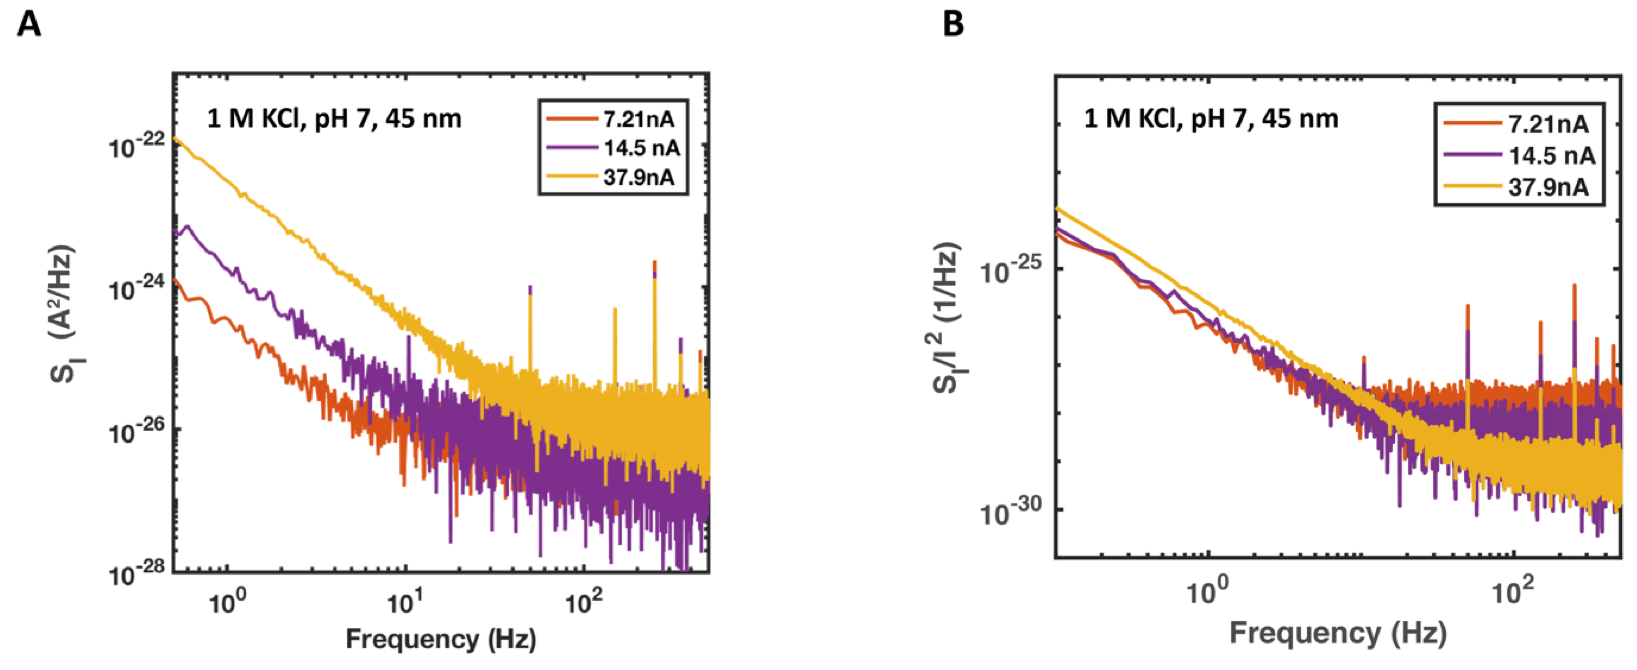
\includegraphics[width=\linewidth]{figures/Figure2.10.png}
	\caption{A. PSD spectra of the ionic current for a 45 nm pore at different bias voltages. B. PSD spectra of the same pore normalized by square of the bias current.}
	\label{fig:fig.2.10}
\end{figure}

\subsection{Example of current trace for a 1.3 nm pore}\label{sec:S2.4.8}

\begin{figure}[!htb]
	\centering
	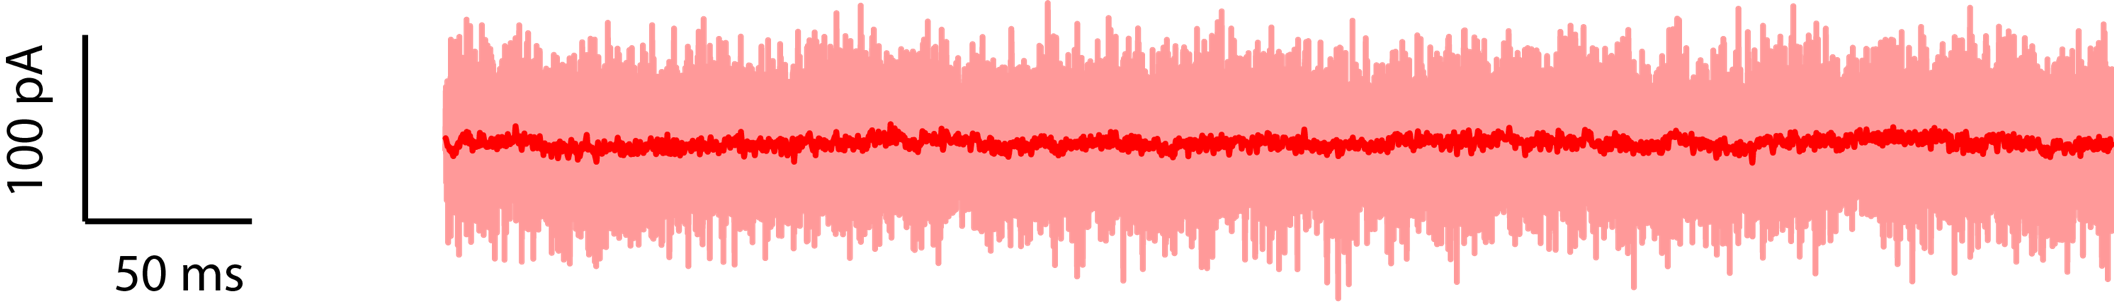
\includegraphics[width=\linewidth]{figures/Figure2.11.png}
	\caption{Example of ionic current trace measured across a small 1.3 nm pore filtered at 10 kHz (light red) and 1 kHz (dark red).}
	\label{fig:fig.2.11}
\end{figure}

\renewcommand{\thefigure}{\thechapter.\arabic{figure}}
\renewcommand{\thetable}{\thechapter.\arabic{table}}
\renewcommand{\theequation}{\thechapter.\arabic{equation}}

\references{chapter-2/chapter-2}

